\documentclass[11pt]{article}
\usepackage[margin=1in]{geometry}
\usepackage{amsmath,amssymb,amsthm}
\usepackage{booktabs}
\usepackage{graphicx}
\usepackage{xcolor}
\usepackage[hidelinks]{hyperref}
\usepackage{enumitem}
\setlist{itemsep=2pt,topsep=4pt}

\newcommand{\R}{\mathbb{R}}
\newcommand{\KL}{\mathrm{KL}}
\newcommand{\TV}{\mathrm{TV}}
\newcommand{\LN}{\mathrm{LN}}
\newcommand{\RT}{\mathcal{R}}
\newtheorem{proposition}{Proposition}

\title{Block Substitution: Measuring What a Trace VAE Round Trip Loses Inside GPT-2}
\author{SpecDec-AF, rev-7}
\date{October 2026}

\begin{document}
\maketitle

\begin{abstract}
We measure the functional cost of a trace VAE's reconstruction error by putting the reconstruction back into the frozen
teacher's forward pass. At a single token position, the output of one transformer block is replaced by its VAE round
trip, and the real model computes everything after it. Divergence from the unmodified run is recorded at every downstream
block and at the final logits. Three controls frame the result: an identity substitution through the same code path, a
size-matched random perturbation, and replacement by the block's dataset mean. Two full-stack variants measure compounding
error and the error of the decoded trace used alone. This note specifies the intervention, metrics, controls,
uncertainty estimates and validation checks, and reports results for the rev-7 model \texttt{rev7B\_optd}.
\end{abstract}

\section{Setup}

\paragraph{Teacher.} GPT-2 small, frozen, in evaluation mode (dropout is the identity). For a token sequence
$x_{1:T}$ and position $p$, write $r_0(p)$ for the token-plus-position embedding and, for blocks $l = 0,\dots,11$,
\begin{align}
  a_l(p) &= \mathrm{Attn}_l\big(\LN_{1,l}(r_l)\big)(p), &
  m_l(p) &= \mathrm{MLP}_l\big(\LN_{2,l}(r_l + a_l)\big)(p), &
  r_{l+1}(p) &= r_l(p) + a_l(p) + m_l(p),
\end{align}
where $a_l$ is the output of the attention output projection (\texttt{attn.c\_proj}) and $m_l$ the output of the MLP output
projection (\texttt{mlp.c\_proj}). The logits are $z(p) = W_U\,\LN_f\big(r_{12}(p)\big)$, and the next-token distribution
is $P(p) = \mathrm{softmax}\,z(p)$. Attention is causal, so $z(p)$ depends only on $x_{1:p}$.

\paragraph{Chunks.} The trace of block $l$ at position $p$ is the chunk $C_l(p) \in \R^{9984}$: eight slots holding
$\LN_{1,l}$ output (768), the QKV projection (2304), $a_l$ (768), $\LN_{2,l}$ output (768), the pre-activation MLP
projection (3072), $m_l$ (768), and two boundary slots. The boundary slots carry $r_0(p)$ at $l = 0$ and
$\LN_f(r_{12}(p))$ at $l = 11$, and are zero elsewhere. We write $\pi_a(C)$ and $\pi_m(C)$ for the $a$ and $m$ slots of
a chunk.

\paragraph{VAE round trip.} The VAE is a single encoder $E$ and decoder $D$ shared across blocks. The decoder is
conditioned only on the block index. With the fixed per-block, per-element normalization
$N_l(C) = (C - \mu_l)/\sigma_l$ and the encoder mean $\mu_E$, the round trip of block $l$ is
\begin{equation}
  \RT_l(C) = D\big(\mu_E(N_l(C)),\, l\big),
\end{equation}
since the decoder emits raw activations (\texttt{decoder\_output\_space: raw}). No latent is sampled. The model evaluated
here is \texttt{rev7B\_optd}: $d_{\text{latent}} = 128$ per block, trained 200k steps on 500{,}768 positions.

\section{Intervention}

\paragraph{Single-position substitution.} An intervention acts at one position $p$ and leaves every other position
unchanged. For a set of active blocks $S \subseteq \{0,\dots,11\}$ and a replacement rule $\phi$ (Section~\ref{sec:conditions}),
the modified forward pass computes, for each block $l$ in order,
\begin{equation}
  \tilde r_{l+1}(p) =
  \begin{cases}
    \tilde r_l(p) + \phi_a\big(\tilde C_l(p)\big) + \phi_m\big(\tilde C_l(p)\big), & l \in S,\\[2pt]
    \tilde r_l(p) + \tilde a_l(p) + \tilde m_l(p), & l \notin S,
  \end{cases}
\end{equation}
with $\tilde r_0 = r_0$. Here $\tilde a_l$, $\tilde m_l$ and the live chunk $\tilde C_l(p)$ are what the real block $l$
computes from the residual it receives in the modified run. In other words, block $l$ runs normally, and if $l \in S$ its
output at $p$ is overwritten before block $l+1$ reads it. Positions $q \neq p$ keep their own residuals, but at $q > p$ they
attend to the modified keys and values at $p$.

\begin{proposition}[Exact localization]
Run the modified forward pass on the prefix $x_{1:p}$. Then the logits at every position $q < p$ equal the unmodified
logits, and the logits at $p$ are exactly the effect of the intervention on the prediction at $p$.
\end{proposition}
\begin{proof}[Sketch]
By causality, the residual at $q < p$ depends only on $x_{1:q}$ and on residuals at positions $\le q$, none of which the
intervention touches. The prediction at $p$ depends only on positions $\le p$, so truncating at $p$ changes nothing.
\end{proof}

\noindent Each modified forward pass therefore perturbs exactly one position. Batches of positions are processed as
independent sequences, right-padded, which by causality does not affect the read-out position.

\paragraph{Live chunks.} The chunk passed to the VAE is assembled from the modified run itself: the six per-block slots
from hooks on the block's submodules, $r_0(p)$ for the input boundary at $l = 0$, and
$\LN_f(\tilde r_{11} + \tilde a_{11} + \tilde m_{11})$ for the output boundary at $l = 11$. In the unmodified run these
equal the cached training chunks up to fp16 storage error (Section~\ref{sec:checks}).

\section{Conditions}
\label{sec:conditions}

\begin{description}[leftmargin=1.2em]
  \item[\texttt{clean}.] No intervention ($S = \varnothing$). All metrics are taken against this run.
  \item[\texttt{vae\_b}.] $S = \{b\}$, $\phi(C) = \big(\pi_a \RT_b(C),\ \pi_m \RT_b(C)\big)$. Blocks before $b$ are
    clean, so the encoder sees the true chunk.
  \item[\texttt{identity\_b}.] $S = \{b\}$, $\phi(C) = (\pi_a C,\ \pi_m C)$: the real values through the same splice.
    This must reproduce \texttt{clean}.
  \item[\texttt{noise\_b}.] $S = \{b\}$, the real values plus isotropic noise with the same norm as the VAE error,
    matched per position and per slot:
    \begin{equation}
      \phi_s(C) = \pi_s C + \big\lVert \pi_s \RT_b(C) - \pi_s C \big\rVert\,\frac{\xi_s}{\lVert \xi_s \rVert},
      \qquad \xi_s \sim \mathcal{N}(0, I_{768}),\quad s \in \{a, m\},
    \end{equation}
    with $\xi_a$ and $\xi_m$ drawn independently from a seeded generator.
  \item[\texttt{meanabl\_b}.] $S = \{b\}$, $\phi = (\bar a_b,\ \bar m_b)$: the means of the two slots at block $b$ over the
    first 10{,}000 training positions. This is a block output that carries no information about the position.
  \item[\texttt{stack\_closed}.] $S = \{0,\dots,11\}$ with the VAE rule. Each block runs on the already-modified residual,
    and its live chunk is round-tripped. This measures compounding, and it feeds the encoder chunks it was not trained on.
  \item[\texttt{stack\_identity}.] $S = \{0,\dots,11\}$ with the identity rule (sanity check).
  \item[\texttt{stack\_open}.] The teacher is never run on reconstructions. The clean chunks of all twelve blocks are
    round-tripped, and the residual stream is rebuilt from decoded values alone:
    \begin{equation}
      \hat r_0 = \pi_{\text{in}} \RT_0(C_0), \qquad
      \hat r_{l+1} = \hat r_l + \pi_a \RT_l(C_l) + \pi_m \RT_l(C_l), \qquad
      \hat z = W_U\, \LN_f(\hat r_{12}).
    \end{equation}
    This is how a trace produced by the latent generator would be read. For reference we also report $W_U$ applied to the
    decoded output-boundary slot of block 11, which is the metric used in the earlier fidelity evaluation.
\end{description}

\section{Metrics}

Let $P$ be the clean next-token distribution at $p$ and $Q$ that of a condition. For each position:
\begin{itemize}
  \item \textbf{Final divergence:} $\KL(P \,\Vert\, Q)$; top-1 agreement $\mathbf{1}[\arg\max P = \arg\max Q]$; top-5
    overlap.
  \item \textbf{Acceptance:} $\alpha(P, Q) = \sum_v \min(P_v, Q_v) = 1 - \TV(P, Q)$, the probability that a token drawn
    from $Q$ is accepted by speculative-decoding verification against $P$. Top-1 agreement is the greedy special case.
    Computed in float64 (fp32 rounding over 50{,}257 tokens is about $10^{-5}$).
  \item \textbf{Cross-entropy:} $\mathrm{CE} = -\log Q(x_{p+1})$ on the true next token, and $\Delta\mathrm{CE}$ against
    clean. The last position of a sequence has no next token and is excluded from these two metrics only.
  \item \textbf{Logit lens at block $l$:} $Q^{(l)} = \mathrm{softmax}\,W_U \LN_f(\tilde r_{l+1}(p))$ against the clean
    $P^{(l)}$; we record $\KL(P^{(l)} \Vert Q^{(l)})$, $\TV$ and top-1 agreement, for every $l$.
  \item \textbf{Residual error:} $\lVert \tilde r_{l+1} - r_{l+1} \rVert / \lVert r_{l+1} \rVert$ and the cosine, for
    every $l$.
  \item \textbf{Chunk error:} per-slot relative error and cosine of the live chunks against clean, for every block and
    every non-padded slot.
\end{itemize}

\paragraph{Derived quantities.} For each block $b$, with $\overline{\KL}_c$ the mean final KL of condition $c$:
\begin{align}
  \rho_b &= \overline{\KL}_{\texttt{vae\_b}} \,/\, \overline{\KL}_{\texttt{noise\_b}}
     && \text{(VAE error versus random error of equal size)},\\
  K_b &= 1 - \overline{\KL}_{\texttt{vae\_b}} \,/\, \overline{\KL}_{\texttt{meanabl\_b}}
     && \text{(share of the position-specific contribution kept)}.
\end{align}
$K_b = 1$ means the reconstruction is as good as the real block output. $K_b = 0$ means it is no better than the block's
mean. The cross-entropy analogue
\begin{equation*}
  \frac{\mathrm{CE}_{\texttt{meanabl}} - \mathrm{CE}_{\texttt{vae}}}{\mathrm{CE}_{\texttt{meanabl}} - \mathrm{CE}_{\texttt{clean}}}
\end{equation*}
is also computed, but it is unstable for the middle blocks (Section~\ref{sec:limits}), and $K_b$ is the quantity we report.

\paragraph{Sample and uncertainty.} The evaluation set is the first $N = 5{,}000$ positions of the pinned validation shards:
313 WikiText-103 sequences of 256 tokens, with 16 positions per sequence drawn uniformly from $[32, 255]$. Positions in one
sequence are correlated, so 95\% intervals come from a cluster bootstrap over sequences: $B = 2{,}000$ resamples of the 313
sequences with replacement. Ratios ($\rho_b$, $K_b$) are recomputed as ratios of resampled sums.

\section{Validation checks}
\label{sec:checks}

\begin{enumerate}
  \item \textbf{Identity is exact.} \texttt{identity\_b} for all $b$, and \texttt{stack\_identity}, give final KL $0$ and
    residual relative error $0$ on all 5{,}000 positions.
  \item \textbf{Live chunks match the cache.} In the clean run, the largest relative difference between hooked chunks
    and the stored training chunks is $2.25 \times 10^{-4}$, the fp16 storage precision.
  \item \textbf{Localization.} A unit test confirms that a substitution at $p$ leaves the logits at all $q < p$
    bit-identical, and changes those at $p$.
  \item \textbf{Hook-free equivalence.} With no active block, the hooked forward pass reproduces a plain forward pass.
  \item \textbf{Acceptance identity.} $\alpha(P, P) = 1$, and $\alpha = 1 - \TV$ on random distribution pairs.
  \item \textbf{Noise matching.} The noise norm equals the VAE error norm per position and per slot (to $10^{-4}$).
\end{enumerate}

\section{Results for \texttt{rev7B\_optd}}

\begin{table}[h]
\centering
\small
\begin{tabular}{rcccccc}
\toprule
Block $b$ & KL vae & KL noise & KL mean & $\rho_b$ [95\% CI] & $K_b$ [95\% CI] & $\alpha$ vae \\
\midrule
0  & 0.255 & 0.022 & 4.37  & 11.8 [10.7, 13.1] & 0.94 [0.94, 0.95] & 0.847 \\
1  & 0.012 & 0.011 & 0.022 & 1.12 [1.03, 1.21] & 0.43 [0.40, 0.46] & 0.958 \\
2  & 0.025 & 0.016 & 0.037 & 1.58 [1.45, 1.73] & 0.32 [0.28, 0.36] & 0.939 \\
3  & 0.033 & 0.019 & 0.039 & 1.72 [1.58, 1.88] & 0.16 [0.12, 0.20] & 0.928 \\
4  & 0.032 & 0.020 & 0.044 & 1.66 [1.50, 1.85] & 0.27 [0.24, 0.30] & 0.926 \\
5  & 0.041 & 0.026 & 0.055 & 1.55 [1.46, 1.64] & 0.27 [0.24, 0.29] & 0.912 \\
6  & 0.047 & 0.032 & 0.063 & 1.50 [1.44, 1.56] & 0.25 [0.23, 0.27] & 0.899 \\
7  & 0.068 & 0.037 & 0.095 & 1.83 [1.76, 1.91] & 0.28 [0.26, 0.30] & 0.876 \\
8  & 0.080 & 0.040 & 0.110 & 1.99 [1.92, 2.07] & 0.27 [0.25, 0.29] & 0.866 \\
9  & 0.102 & 0.049 & 0.134 & 2.06 [1.99, 2.13] & 0.24 [0.22, 0.26] & 0.847 \\
10 & 0.134 & 0.067 & 0.168 & 2.01 [1.94, 2.10] & 0.20 [0.19, 0.21] & 0.826 \\
11 & 0.209 & 0.264 & 0.368 & 0.79 [0.76, 0.82] & 0.43 [0.42, 0.45] & 0.784 \\
\bottomrule
\end{tabular}
\caption{Single-block substitution. Mean final $\KL(P\Vert Q)$ for the VAE, size-matched noise and mean replacement;
VAE-to-noise ratio $\rho_b$; share kept $K_b$; and VAE acceptance $\alpha$. $N = 5{,}000$ positions, 313 sequences.}
\label{tab:single}
\end{table}

\begin{table}[h]
\centering
\small
\begin{tabular}{lcccc}
\toprule
Condition & KL [95\% CI] & $\alpha$ & top-1 \\
\midrule
\texttt{stack\_closed} & 2.38 [2.31, 2.45] & 0.378 & 0.268 \\
\texttt{stack\_open}   & 1.46 [1.41, 1.51] & 0.508 & 0.398 \\
decoded block-11 output slot $\to W_U$ & 0.89 & 0.619 & 0.518 \\
\bottomrule
\end{tabular}
\caption{Full-stack conditions.}
\label{tab:stack}
\end{table}

\begin{figure}[h]
\centering
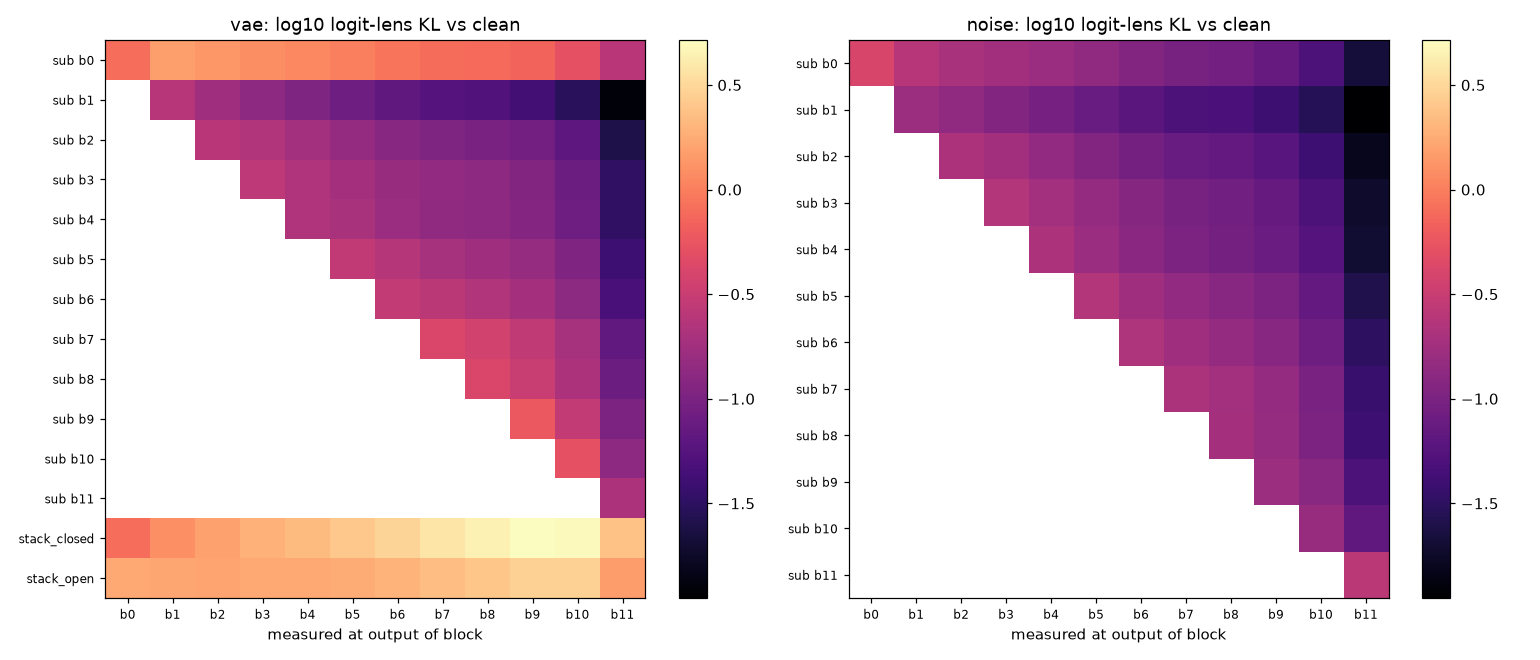
\includegraphics[width=\linewidth]{figures/grid_lens_kl.png}
\caption{Logit-lens $\log_{10}\KL$ against clean. Rows: substituted block (and the two full-stack conditions). Columns:
block whose output is read. Left: VAE; right: size-matched noise; shared colour scale.}
\label{fig:grid}
\end{figure}

\begin{figure}[h]
\centering
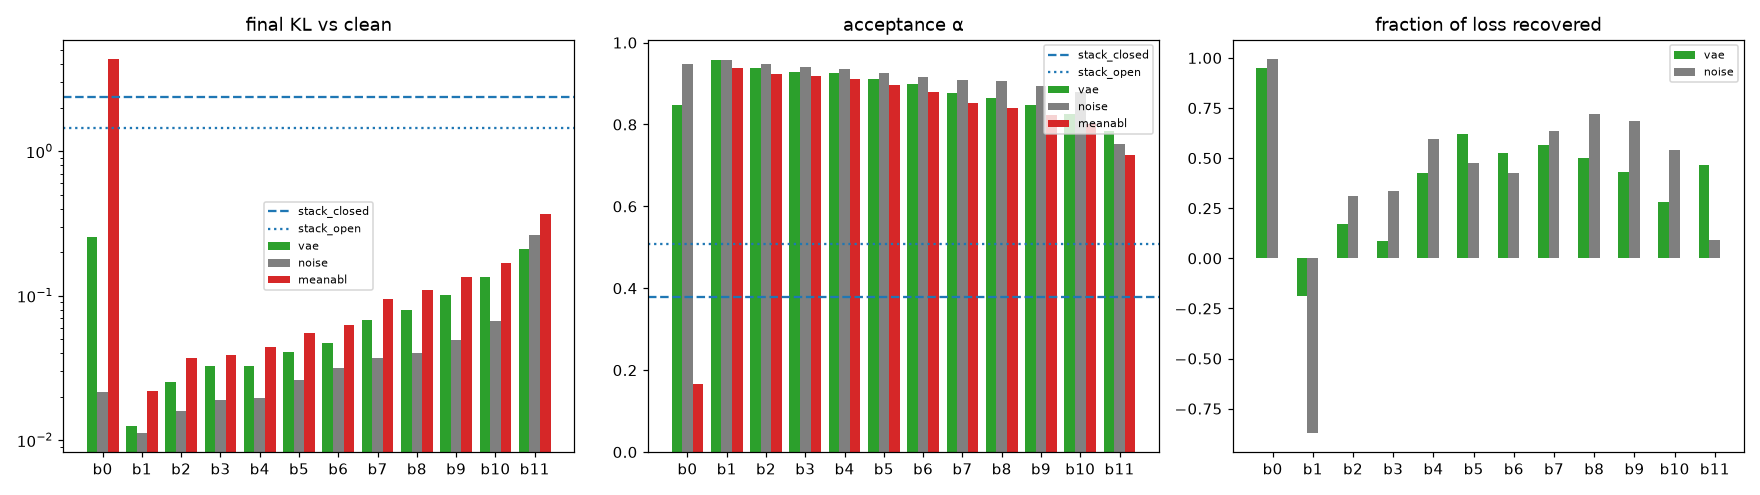
\includegraphics[width=\linewidth]{figures/per_block_final.png}
\caption{Per-block final KL (log scale), acceptance, and the cross-entropy recovery ratio (unstable; see
Section~\ref{sec:limits}).}
\label{fig:bars}
\end{figure}

\begin{figure}[h]
\centering
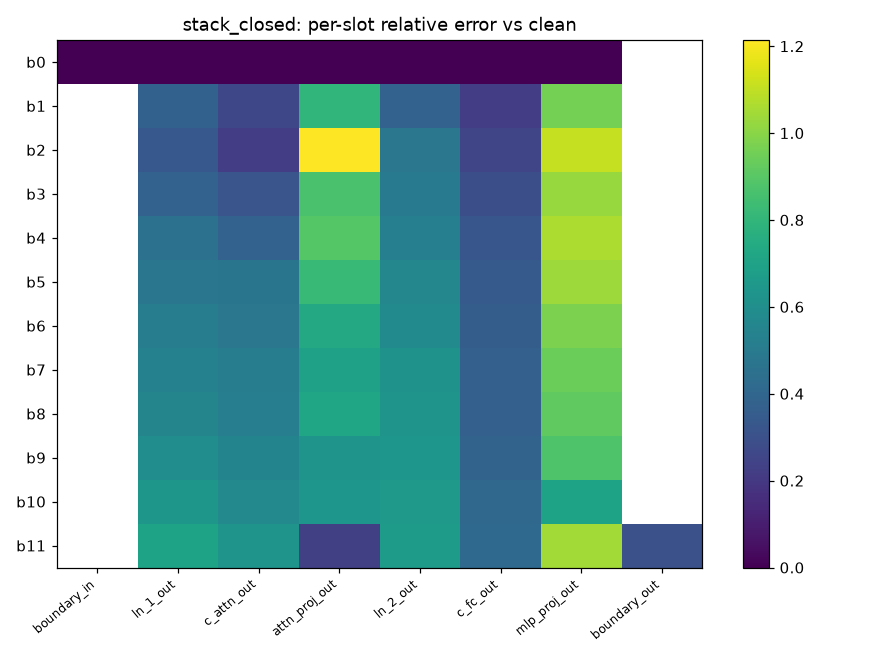
\includegraphics[width=0.62\linewidth]{figures/stack_closed_slots.png}
\caption{\texttt{stack\_closed}: per-slot relative error of the live chunks against clean, by block.}
\label{fig:slots}
\end{figure}

\paragraph{Summary.}
\begin{enumerate}
  \item A single-block substitution changes the prediction little: $\alpha$ between 0.78 and 0.96.
  \item The VAE error is more damaging than size-matched isotropic noise at blocks 2--10 ($\rho_b \approx 1.5$--$2.1$) and
    much more at block 0 ($\rho_0 = 11.8$). Its error is concentrated in directions the teacher is sensitive to.
  \item Measured against mean replacement, the reconstruction keeps $K_b = 0.16$--$0.43$ of the position-specific
    contribution of blocks 1--11. At block 0, $K_0 = 0.94$ only because mean replacement erases token identity
    ($\KL = 4.37$); in absolute terms block 0 is the worst single block.
  \item Single-block divergence peaks at the substituted block and falls by a factor of 6--20 by the output, for both
    VAE and noise (Figure~\ref{fig:grid}).
  \item With substitution at every block (\texttt{stack\_closed}), logit-lens divergence grows steadily with depth and
    the final KL is 2.38. This is worse than the decoded trace read on its own (\texttt{stack\_open}, 1.46).
\end{enumerate}

\section{Limitations}
\label{sec:limits}

\begin{itemize}
  \item \textbf{Slots tested.} A single-block substitution uses only the two residual-writing slots, $a_b$ and $m_b$.
    Errors in the LayerNorm, QKV and pre-activation slots do not enter, because the teacher recomputes them. Those slots
    are assessed only by direct reconstruction error and the weight-consistency identities. \texttt{stack\_open} also
    uses the input boundary slot.
  \item \textbf{One position at a time.} A generated sequence would perturb every position, including the keys and
    values that later positions attend to. These results are a lower bound for that case. Multi-position substitution
    needs a cache with every position of each sequence.
  \item \textbf{Cross-entropy recovery ratio.} For blocks 1--10, mean replacement raises the cross-entropy by only
    0.01--0.14 nats. The CE ratio's denominator is then close to zero and the estimate is unstable, even negative.
    $K_b$, which uses KL, does not have this problem.
  \item \textbf{Isotropic noise.} The noise control spreads energy evenly over all 768 directions. The teacher's
    sensitivity is strongly anisotropic, so this is a conventional but weak baseline. Noise drawn from each slot's
    empirical covariance, or projected onto the decoder's error subspace, would give a stricter comparison.
  \item \textbf{Residual relative error.} The residual norm grows with depth, so a fixed error shrinks in relative terms
    downstream. The logit-lens KL is the better measure of propagation.
  \item \textbf{Logit lens in early blocks.} The logit lens is a coarse read-out of GPT-2's early layers. Compare VAE and
    noise within a block; avoid comparing absolute logit-lens values across blocks.
  \item \textbf{Mean latent only.} The round trip uses the encoder mean. In the rev-7 fidelity evaluation, sampled
    latents were within 0.2 percentage points of the mean on top-1 agreement.
  \item \textbf{Off-distribution inputs in \texttt{stack\_closed}.} Under compounding, the encoder sees chunks computed
    from perturbed residuals. That condition combines decoder error with encoder robustness, and the two are not
    separated here.
\end{itemize}

\section{Reproducibility}

Code: \texttt{specdec\_af/analysis/substitution.py} (commit \texttt{56fbefa}; plot colour-scale fix
\texttt{b6dabbc}). Tests: \texttt{tests/test\_substitution.py}. The run took 33 minutes on one V100-SXM2
(Explorer job 11081685):
\begin{verbatim}
RUN_NAME=rev7B_optd DUMP_RESIDUALS=1 sbatch scripts/slurm/submit_substitution.sh
\end{verbatim}
Outputs: \texttt{metrics.json}, \texttt{summary.txt}, \texttt{per\_position.npz} (final KL, $\alpha$, $\Delta$CE and top-1
per position and condition), \texttt{block\_means.pt}, the figures, and residual dumps
$[N, 13, 768]$ in fp16 for the clean, single-block VAE and full-stack conditions (input to a planned SAE feature
analysis).

\end{document}
